\documentclass[conference]{IEEEtran}
\usepackage{times}
\usepackage[numbers]{natbib}
\usepackage{multicol}
\usepackage{amsmath,amssymb,amsfonts}
\usepackage{graphicx}
\usepackage{booktabs}
\usepackage{tabularx}
\usepackage{multirow}
\usepackage{microtype}
\let\labelindent\relax
\usepackage{enumitem}
\setlist{noitemsep, topsep=1.5pt, leftmargin=*}
\usepackage{xcolor}
\usepackage{tikz}
\usetikzlibrary{shapes.geometric, arrows.meta, positioning, calc, backgrounds, fit}
\usepackage[bookmarks=true,hidelinks]{hyperref}

% Define color palette
\definecolor{brandblue}{RGB}{31, 78, 121}
\definecolor{brandred}{RGB}{192, 0, 0}
\definecolor{brandgreen}{RGB}{56, 124, 68}
\definecolor{brandamber}{RGB}{197, 90, 17}
\definecolor{brandpurple}{RGB}{112, 48, 160}
\definecolor{brandteal}{RGB}{0, 128, 128}
\definecolor{brandslate}{RGB}{80, 80, 80}
\definecolor{boxbg}{RGB}{245, 247, 250}

% Pre-submission marker: every \TODO must be resolved (or the macro emptied) before the Stage 1 freeze.
\newcommand{\TODO}[1]{\textcolor{red}{\textbf{[TODO: #1]}}}
\newcommand{\TBD}{\textcolor{red}{\textbf{TBD}}}

\pdfinfo{
   /Author (Anonymous)
   /Title  (AFFORD-Bench: An Affordance-Grounded Benchmark and Generalization Evaluation for Robot Learning)
   /Subject (Robotics Benchmarks, Imitation Learning, Out-of-Distribution Generalization, Affordance Grounding)
   /Keywords (Robot Manipulation; Vision-Language-Action Models; Affordance Grounding; Out-of-Distribution Benchmark)
}

\begin{document}

\title{AFFORD-Bench: An Affordance-Grounded Benchmark and Generalization Evaluation for Robot Learning}

\author{Author Names Omitted for Anonymous Review. Paper-ID [RSS-2027-0150]}

\maketitle

\begin{abstract}
Imitation learning policies and Vision-Language-Action (VLA) models report high success on standard manipulation benchmarks, yet LIBERO-PRO and LIBERO-X show that these numbers collapse under modest changes to object layout, appearance, or instruction wording, which points to memorization of nominal scenes. Existing robustness suites perturb mostly tabletop pick-and-place scenes and rarely vary the quantities that set whether a contact-rich task can succeed: placement tolerance, friction, and mass. We introduce \textbf{AFFORD-Bench}, a policy-agnostic MuJoCo benchmark with \textbf{210 tasks} across \textbf{7 domains} (industrial assembly, culinary, domestic tabletop, laboratory, long-horizon, precision chains, and service chains) on a simulated Franka Emika Panda. It ships oracle demonstrations with dual-camera RGB ($640\times 660$ workcell, $300\times 420$ wrist), optional metric depth, and proprioception in Robomimic HDF5, together with four instruction variants per task (metric, contact-conditioned, terse, and subtask-decomposed). We specify a five-level perturbation hierarchy (L1--L5) over spatial, photometric, physical, and compound shifts, organized as 35 evaluation suites, and we state which parts are implemented in this Stage 1 release and which belong to the Stage 2 Extension Charter.
\end{abstract}

\IEEEpeerreviewmaketitle

\section{Introduction}
\label{sec:intro}

Generalist Vision-Language-Action (VLA) models~\cite{kim2024openvla, octo2023, padalkar2023openx}, compact VLAs such as SmolVLA~\cite{smolvla2025}, subtask-aware post-training such as AtomVLA~\cite{atomvla2025}, and action-chunking visuomotor policies~\cite{chi2023diffusion, zhao2023act} all promise transfer across tasks and scenes.

Measuring that transfer remains difficult. LIBERO~\cite{liu2023libero} is the de facto testbed, but \citet{zhou2026liberopro} (LIBERO-PRO) and \citet{wang2026liberox} (LIBERO-X) show that policies exceeding 90\% nominal success can fall to near 0\% under small spatial offsets, object swaps, or altered instructions, and attribute the gap to memorized trajectories and layouts.

\begin{figure}[t]
\centering
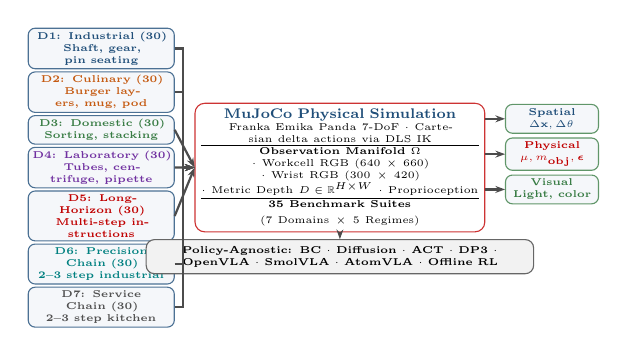
\begin{tikzpicture}[
    scale=0.72, every node/.style={transform shape},
    domainbox/.style={rectangle, rounded corners=2.5pt, draw=brandblue!80, fill=boxbg, inner sep=1.8pt, text width=2.45cm, align=center, font=\tiny\bfseries},
    corebox/.style={rectangle, rounded corners=3.5pt, draw=brandred!80, fill=white, inner sep=3.0pt, text width=4.9cm, align=center, font=\scriptsize},
    axisbox/.style={rectangle, rounded corners=2.5pt, draw=brandgreen!80, fill=boxbg, inner sep=2.0pt, text width=1.5cm, align=center, font=\tiny\bfseries},
    arr/.style={-{Stealth[length=3.5pt,width=2.5pt]}, thick, draw=black!70}
]
    % Domains column (7 domains)
    \node[domainbox] (d1) {\color{brandblue}D1: Industrial (30)\\ \tiny Shaft, gear, pin seating};
    \node[domainbox, below=1.2pt of d1] (d2) {\color{brandamber}D2: Culinary (30)\\ \tiny Burger layers, mug, pod};
    \node[domainbox, below=1.2pt of d2] (d3) {\color{brandgreen}D3: Domestic (30)\\ \tiny Sorting, stacking};
    \node[domainbox, below=1.2pt of d3] (d4) {\color{brandpurple}D4: Laboratory (30)\\ \tiny Tubes, centrifuge, pipette};
    \node[domainbox, below=1.2pt of d4] (d5) {\color{brandred}D5: Long-Horizon (30)\\ \tiny Multi-step instructions};
    \node[domainbox, below=1.2pt of d5] (d6) {\color{brandteal}D6: Precision Chain (30)\\ \tiny 2--3 step industrial};
    \node[domainbox, below=1.2pt of d6] (d7) {\color{brandslate}D7: Service Chain (30)\\ \tiny 2--3 step kitchen};

    % Core Engine (aligned with middle domain D4)
    \node[corebox, right=10pt of d4] (sim) {
        \textbf{\color{brandblue}MuJoCo Physical Simulation}\\
        \tiny Franka Emika Panda 7-DoF $\cdot$ Cartesian delta actions via DLS IK\\
        \vspace{1pt}\hrule\vspace{1pt}
        \textbf{Observation Manifold $\Omega$}\\
        $\cdot$ Workcell RGB ($640\times 660$) $\cdot$ Wrist RGB ($300\times 420$)\\
        $\cdot$ Metric Depth $D \in \mathbb{R}^{H\times W}$ $\cdot$ Proprioception\\
        \vspace{1pt}\hrule\vspace{1pt}
        \textbf{35 Benchmark Suites} ($7 \text{ Domains} \times 5 \text{ Regimes}$)
    };

    % Perturbation axes
    \node[axisbox, right=10pt of sim.north east, yshift=-8pt] (p_spat) {\color{brandblue}Spatial\\ \tiny $\Delta \mathbf{x}, \Delta\theta$};
    \node[axisbox, below=2pt of p_spat] (p_phys) {\color{brandred}Physical\\ \tiny $\mu, m_{\text{obj}}, \boldsymbol{\epsilon}$};
    \node[axisbox, below=2pt of p_phys] (p_vis) {\color{brandgreen}Visual\\ \tiny Light, color};

    % Policy baselines
    \node[rectangle, rounded corners=3pt, draw=black!60, fill=gray!10, text width=6.6cm, align=center, font=\tiny\bfseries, below=3.5pt of sim] (policy) {
        Policy-Agnostic: BC $\cdot$ Diffusion $\cdot$ ACT $\cdot$ DP3 $\cdot$ OpenVLA $\cdot$ SmolVLA $\cdot$ AtomVLA $\cdot$ Offline RL
    };

    % Connectors
    \draw[arr] (d1.east) -- ++(4pt,0) |- (sim.west);
    \draw[arr] (d2.east) -- ++(4pt,0) |- (sim.west);
    \draw[arr] (d3.east) -- (sim.west);
    \draw[arr] (d4.east) -- (sim.west);
    \draw[arr] (d5.east) -- (sim.west);
    \draw[arr] (d6.east) -- ++(4pt,0) |- (sim.west);
    \draw[arr] (d7.east) -- ++(4pt,0) |- (sim.west);

    \draw[arr] (sim.east |- p_spat) -- (p_spat.west);
    \draw[arr] (sim.east |- p_phys) -- (p_phys.west);
    \draw[arr] (sim.east |- p_vis) -- (p_vis.west);

    \draw[arr] (sim.south) -- (policy.north);
\end{tikzpicture}
\caption{\textbf{The AFFORD-Bench Architecture.} 210 tasks in 7 domains, evaluated under spatial, physical, and visual shifts in 35 suites.}
\label{fig:teaser}
\end{figure}

LIBERO-PRO and LIBERO-X perturb layout, appearance, and language; COLOSSEUM~\cite{pumacay2024colosseum} adds physical-property axes over 20 RLBench tasks. None of them couples these shifts to the quantity that decides success in precision work: how much positional error the task tolerates. In the sense of affordance theory~\cite{gibson1979ecological}, whether a part can be seated depends jointly on clearance, friction, and mass, not on appearance alone. Contact-rich assembly simulators such as Factory~\cite{narang2022factory} and IndustReal~\cite{tang2023industreal} model these effects with high fidelity but target reinforcement learning on a few assemblies, not cross-domain evaluation of imitation and VLA policies.

A benchmark should also be \textbf{policy-agnostic}: usable by behavior cloning, chunked diffusion and transformer policies (Diffusion Policy, ACT), point-cloud policies (DP3), VLAs (OpenVLA, SmolVLA, AtomVLA), and offline reinforcement learning (CQL, IQL).

AFFORD-Bench contributes:
\begin{enumerate}
    \item \textbf{Task scale and domain spread}: \textbf{210 tasks} in \textbf{7 domains}, spanning industrial seating, culinary stacking, tabletop sorting, laboratory handling, and multi-step instructions.
    \item \textbf{Policy-agnostic data}: dual-camera RGB ($640\times 660$ workcell, $300\times 420$ wrist), optional metric depth, joint and Cartesian proprioception, and success flags in Robomimic HDF5~\cite{mandlekar2021robomimic}, convertible to RLDS and LeRobot formats.
    \item \textbf{Hierarchical perturbations}: a five-level hierarchy (L1 nominal, L2 spatial, L3 visual, L4 physical, L5 compound) yielding \textbf{35 suites}, with an explicit implementation status per level (Sec.~\ref{sec:perturbations}).
    \item \textbf{Multi-tier language}: four instruction variants per task (metric, contact-conditioned, terse, and subtask-decomposed with pre/post predicates), each annotated with whether the simulator evaluates what it asks.
\end{enumerate}

\begin{figure*}[t]
\centering
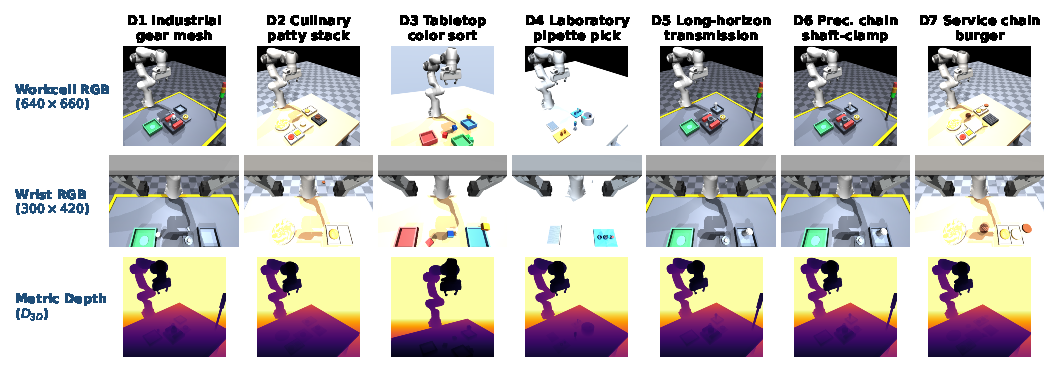
\includegraphics[width=\linewidth, height=3.4cm]{figures/tasks_horizontal_vis.pdf}
\caption{\textbf{Multi-Domain Qualitative Visualizations in AFFORD-Bench.} Representative tasks from all seven domains: (Row 1) workcell RGB ($640\times 660$); (Row 2) wrist RGB ($300\times 420$); (Row 3) metric depth rendered from the workcell camera (meters).}
\label{fig:tasks_vis}
\end{figure*}

\section{Related Work}
\label{sec:related}

\subsection{Robotic Manipulation Benchmarks}
RLBench~\cite{james2020rlbench} and ManiSkill2~\cite{gu2023maniskill2} provide simulated suites for reinforcement and demonstration-guided learning. Robomimic~\cite{mandlekar2021robomimic} standardized offline imitation learning pipelines across demonstration qualities. LIBERO~\cite{liu2023libero} introduced 130 tasks for lifelong knowledge transfer. These suites evaluate mostly nominal execution without systematic out-of-distribution (OOD) testing.

\subsection{OOD Robustness and Modern VLA Architectures}
With large-scale pretrained policies~\cite{padalkar2023openx, brohan2022rt1, brohan2023rt2, kim2024openvla, octo2023}, robustness to distribution shift has become a primary question. LIBERO-PRO~\cite{zhou2026liberopro} shows that policies with high nominal LIBERO success collapse under perturbed objects, initial states, and instructions. LIBERO-X~\cite{wang2026liberox} adds hierarchical, cumulative perturbation levels. COLOSSEUM~\cite{pumacay2024colosseum} varies 14 factors, including physical properties, and reports 30--50\% degradation for single factors and at least 75\% for combined ones. SmolVLA~\cite{smolvla2025} pairs a compact vision-language backbone with a flow-matching action expert for low-cost hardware, and AtomVLA~\cite{atomvla2025} combines subtask decomposition with a predictive latent world model for offline post-training. These evaluations remain concentrated on domestic tabletop scenes with loose placement tolerances.

\subsection{Affordance and Contact-Rich Manipulation}
Affordance theory~\cite{gibson1979ecological} frames objects by the interactions they permit. In robotics this has motivated contact-rich grasping~\cite{song2023grasping}, spatial affordance maps~\cite{shridhar2022cliport}, and 3D policy representations such as DP3~\cite{ze2024dp3}. Factory~\cite{narang2022factory} and IndustReal~\cite{tang2023industreal} simulate contact-rich assembly with SDF collisions and transfer RL insertion and gear-meshing policies to a real Franka. Diffusion Policy~\cite{chi2023diffusion} and ACT~\cite{zhao2023act} reach high precision on low-cost hardware~\cite{fu2024mobilealoha}, but how they degrade as tolerance tightens or friction changes is not characterized at scale. Offline RL~\cite{kumar2020cql} additionally needs transitions and rewards that VLA-specific datasets often omit. AFFORD-Bench targets this combination of tolerance-indexed tasks, multi-domain coverage, and policy-agnostic data.

\section{The AFFORD-Bench Formulation}
\label{sec:benchmark}

\subsection{Tasks as Goal-Conditioned MDPs}
Each task is a tuple $\kappa = (\ell, \mathbf{e}, \mathcal{C}_{\text{aff}})$ with instruction $\ell$, environment $\mathbf{e} = (\mathcal{W}, \mathcal{O}, \rho_0, \Phi)$, and goal set $\mathcal{C}_{\text{aff}}$. $\mathcal{W}$ is the workspace geometry, $\mathcal{O} = \{o_1, \dots, o_K\}$ the object set with one evaluated body $o^\star \in \mathcal{O}$, $\rho_0$ the initial-state distribution, and $\Phi = (\mu, m, \boldsymbol{\epsilon})$ the physical parameters: sliding friction $\mu$ of $o^\star$, its mass $m$, and success tolerance $\boldsymbol{\epsilon} = (\epsilon_{xy}, \epsilon_z)$.

Each task induces an MDP $\mathcal{M} = \langle \mathcal{S}, \mathcal{A}, P, R, \Omega, H \rangle$. $\mathcal{S}$ is the joint robot-object state. An action $\mathbf{a} = (\Delta\mathbf{p}, \Delta\boldsymbol{\theta}, a_{\text{grip}}) \in [-1,1]^7$ commands a TCP position increment $0.025\,\Delta\mathbf{p}$\,m, capped at 2.5\,cm per step (0.5\,m/s) and tracked by damped-least-squares IK at 20\,Hz, a rotation increment $\Delta\boldsymbol{\theta}$ (reserved and not executed in Stage 1), and a gripper opening $w = 0.02\,(a_{\text{grip}} + 1)$\,m per finger. $P(s' \mid s, \mathbf{a})$ is given by MuJoCo~\cite{todorov2012mujoco} and is deterministic given $s$; all stochasticity enters through $\rho_0$ and the perturbation sampler, both seeded per episode. $R(s) = \mathbb{I}[s \in \mathcal{C}_{\text{aff}}]$ is sparse, and $H$ is the step budget.

The goal set is a state set:
\begin{align}
\mathcal{C}_{\text{aff}} = \big\{ s \in \mathcal{S} \;\big|\; & \|\mathbf{p}^{xy}_{o^\star} - \mathbf{p}^{xy}_{\text{goal}}\|_2 \le \epsilon_{xy}, \notag \\
& |p^{z}_{o^\star} - p^{z}_{\text{goal}}| \le \epsilon_z, \; w \ge w_{\text{rel}} \big\},
\end{align}
with release threshold $w_{\text{rel}} = 0.03$\,m. Four lift-and-replace tasks also require $o^\star$ to have been raised by $h_{\min} \in [0.10, 0.15]$\,m before placement. For reach-and-press tasks the condition is $\|\mathbf{p}_{\text{tcp}} - \mathbf{p}_{\text{goal}}\|_2 \le 0.025$\,m. Episodes terminate at the first $t \le H$ with $s_t \in \mathcal{C}_{\text{aff}}$, so policy competence is
\begin{equation}
J(\pi; \kappa) = \mathbb{P}_{s_0 \sim \rho_0,\; \tau \sim \pi}\big[\exists\, t \le H : s_t \in \mathcal{C}_{\text{aff}}\big].
\end{equation}
Contact forces are monitored, not part of success: an episode violates safety if $\|\mathbf{f}_c(s_t)\| > F_{\max}$ for some $t$, with $F_{\max}$ \TODO{set per domain}.

\subsection{Policy-Agnostic Benchmark Architecture}
The observation $\mathbf{o}_t \in \Omega$ comprises:
\begin{enumerate}
    \item \textbf{Workcell RGB}: $H \times W = 640 \times 660$, uint8;
    \item \textbf{Wrist RGB}: $300 \times 420$, uint8, mounted at the gripper;
    \item \textbf{Metric depth} (optional): float32 $D \in \mathbb{R}^{640 \times 660}$ in meters, back-projected as $\mathbf{P} = D(u,v)\,\mathbf{K}^{-1} [u, v, 1]^\top$ using the stored camera intrinsics $\mathbf{K}$ \TODO{store $\mathbf{K}$ and enable depth in the generator};
    \item \textbf{Proprioception}: joint positions $\mathbf{q} \in \mathbb{R}^7$, velocities $\dot{\mathbf{q}} \in \mathbb{R}^7$, TCP pose $\mathbf{x}_{\text{tcp}} \in \mathbb{R}^7$ (position and $w$-first quaternion), and per-finger opening $w \in [0, 0.04]$\,m;
    \item \textbf{Rewards and termination}: per-step sparse reward $R(s_t)$ and success flag.
\end{enumerate}

\begin{table*}[t]
\centering
\caption{\textbf{Taxonomy of the AFFORD-Bench Suite.} 210 tasks in 7 domains. Tolerances are the success thresholds $(\epsilon_{xy}, \epsilon_z)$ of the Stage 1 release; tolerance-indexed variants are a Stage 2 deliverable.}
\label{tab:domains}
\scriptsize
\setlength{\tabcolsep}{2.5pt}
\renewcommand{\arraystretch}{0.91}
\begin{tabularx}{\linewidth}{lccXXc}
\toprule
\textbf{Domain} & \textbf{Task IDs} & \textbf{Count} & \textbf{Representative Manipulation Tasks} & \textbf{Evaluated Bodies} & \textbf{Tol. ($\epsilon_{xy}$/$\epsilon_z$, mm)} \\
\midrule
\textbf{D1: Industrial Precision} & 001--030 & 30 & Shaft-in-bore, gear-on-shaft, pin-in-hole, kitting, fixture contact & Shaft, spur gear, dowel pin & 30--40 / 20--30 \\
\textbf{D2: Culinary Operations} & 031--060 & 30 & Burger layer stacking, mug to drip tray, capsule to hopper & Patty, cheese, tomato, buns, mug, capsule & 35--40 / 25--30 \\
\textbf{D3: Domestic Tabletop} & 061--090 & 30 & Color sorting, block stacking, relocation, touch & Two cubes, one cylinder & 40 / 30 \\
\textbf{D4: Laboratory Sciences} & 091--120 & 30 & Tube racking, centrifuge loading, pipette positioning & Conical tube, microtube, pipette & 10--40 / 30 \\
\textbf{D5: Long-Horizon Sequences} & 121--150 & 30 & Multi-step assembly, sorting, and service instructions & One per task (Stage 1) & 40 / 30 \\
\textbf{D6: Precision Chaining} & 151--180 & 30 & 2--3 step industrial and laboratory chains & One per task (Stage 1) & 40 / 30 \\
\textbf{D7: Service Assembly} & 181--210 & 30 & 2--3 step kitchen and household chains & One per task (Stage 1) & 40 / 30 \\
\midrule
\textbf{Total} & \textbf{001--210} & \textbf{210} & \textbf{7 Domains $\times$ 30 Tasks (35 Evaluation Suites)} & \textbf{16 rigid bodies} & \textbf{10--40 / 20--30} \\
\bottomrule
\end{tabularx}
\end{table*}

\subsection{Domain Architecture}
As summarized in Table~\ref{tab:domains} and Figure~\ref{fig:tasks_vis}, AFFORD-Bench has seven domains of 30 tasks each across five scenes:
\textbf{D1: Industrial Precision} (001--030): shaft, gear, and pin seating in a jig, kitting, and fixture contact.
\textbf{D2: Culinary Operations} (031--060): burger layer stacking, mug and capsule handling at an espresso station.
\textbf{D3: Domestic Tabletop} (061--090): color sorting into bins, stacking, and relocation.
\textbf{D4: Laboratory Sciences} (091--120): tube racking, centrifuge loading, and pipette positioning.
\textbf{D5--D7} (121--210): instructions that chain 2--4 steps across industrial, laboratory, and kitchen scenes. In Stage 1 each of these tasks evaluates a single body, and the episode ends when that body reaches its goal, which in 57 of 90 tasks occurs before the last instructed step. Multi-body sequential predicates that score every step are a Stage 2 deliverable.

\section{The Hierarchical Affordance Perturbation Framework}
\label{sec:perturbations}

AFFORD-Bench organizes distribution shift into five levels:

\textbf{L1: Nominal (in-distribution).} Default scene; the initial positions of $o^\star$ and the TCP are jittered by $\pm 1.5$\,cm per horizontal axis and the yaw of $o^\star$ by $\pm 15^\circ$, sampled from the episode seed.

\textbf{L2: Spatial ($\mathcal{P}_{\mathrm{spatial}}$).} $\mathbf{p}_{\text{init}} \sim \mathcal{U}(\mathbf{p}_0 - \boldsymbol{\delta}, \mathbf{p}_0 + \boldsymbol{\delta})$ with $\boldsymbol{\delta} = [0.03, 0.03, 0]^\top$\,m and yaw $\theta \sim \mathcal{U}(-45^\circ, 45^\circ)$, probing closed-loop servoing versus trajectory recall.

\textbf{L3: Visual ($\mathcal{P}_{\mathrm{visual}}$).} Light intensity in $[0.5, 1.5]\,I_0$, light position jitter of $\pm 0.5\,\text{m}$, and object color jitter of $\pm 25\%$, leaving geometry unchanged. Lights and colors are restored to nominal before each sample.

\textbf{L4: Physical ($\mathcal{P}_{\mathrm{physics}}$).} Sliding friction $\mu \sim \mathcal{U}(0.10, 1.20)$ and mass $m \sim \mathcal{U}(0.5, 3.0)\,m_0$ of $o^\star$ at identical visual coordinates. \TODO{implement; requires contact-based grasping, since Stage 1 attaches grasped bodies kinematically to the TCP}

\textbf{L5: Compound ($\mathcal{P}_{\mathrm{comp}}$).} L2, L3, and L4 sampled jointly, combined with the multi-step instructions of D5--D7.

\textbf{Implementation status.} In the Stage 1 release, L1, L2, L3, and object-color shifts are implemented; L5 currently combines L2, L3, and color. At reset, bodies are lifted out of any spawn interpenetration and simulated until at rest (at least 40 physics steps) before the first observation. Grasped bodies are rigidly attached to the TCP, and a release within 4.5--6\,cm of the goal seats the body at the goal pose until it is grasped again. Stage 1 results therefore measure spatial and photometric generalization of goal-reaching, not contact dynamics.

\section{Algorithmic Oracles and Dataset Synthesis}
\label{sec:oracles}

\subsection{Scripted Waypoint Oracles}
Teleoperated demonstrations are costly and inconsistent~\cite{mandlekar2021robomimic}. AFFORD-Bench instead uses scripted oracles: from the settled reset pose of $o^\star$, each oracle builds a fixed sequence of approach, grasp, lift, transfer, place, and retract waypoints, interpolates them with a smoothstep profile, and tracks them with the same IK controller used by learned policies. The waypoints are planned once per episode, so the oracle is open-loop with respect to object motion after reset.

\subsection{Demonstration Scale and Packaging}
The generator records 50 demonstrations per task, 10,500 in total and over $2.2 \times 10^6$ timesteps, in Robomimic HDF5 with 90\%/10\% train/validation masks and per-episode metadata. Each demonstration is generated from its own seed, so the 50 demonstrations of a task start from distinct layouts \TODO{regenerate the dataset with the 20\,Hz controller and update the timestep count}. Conversion to RLDS (OpenVLA, Octo) and LeRobot (SmolVLA) formats is required for VLA training.

\section{Training and Evaluation Protocols}
\label{sec:protocols}

\subsection{Standardized Closed-Loop Rollout Procedure}
Each policy step applies one action at 20\,Hz: the arm is interpolated to the IK joint target over 25 physics steps of 2\,ms, with commanded TCP speed capped at 0.5\,m/s. For each task we roll out $N=50$ episodes with evaluation seeds disjoint from data-generation seeds, with $H=400$ steps for D1--D4 and $H=800$ for D5--D7. Every suite, including nominal, draws its initial state from the evaluation seed.

\subsection{Standardized Evaluation Suites}
Models are evaluated on 35 suites (7 domains $\times$ 5 conditions): (1)~\textbf{Nominal}; (2)~\textbf{Spatial} ($\mathcal{P}_{\mathrm{spatial}}$); (3)~\textbf{Visual} ($\mathcal{P}_{\mathrm{visual}}$); (4)~\textbf{Physical} ($\mathcal{P}_{\mathrm{physics}}$); and (5)~\textbf{Composite} ($\mathcal{P}_{\mathrm{comp}}$), with parameters as in Sec.~\ref{sec:perturbations}. Language variants are evaluated as a separate axis on the nominal scene.

\subsection{Quantitative Evaluation Metrics}
We report: (i)~\textbf{Success Rate} $\text{SR} = \frac{1}{N} \sum_{i=1}^N \mathbb{I}[\exists\, t \le H : s^{(i)}_t \in \mathcal{C}_{\text{aff}}]$ with Wilson 95\% intervals over episodes and mean $\pm$ s.d. over 3 training seeds; (ii)~\textbf{Physical Robustness Index} $\text{PRI}(\mathcal{P}) = \text{SR}(\mathcal{P}) / \text{SR}(\text{Nominal}) \times 100\%$, defined when $\text{SR}(\text{Nominal}) > 0$; (iii)~\textbf{Generalization Degradation Index} $\text{GDI} = 100\% - \text{PRI}$; and (iv)~\textbf{Force Violation Rate} (FVR), the fraction of episodes violating $F_{\max}$.

\section{Scientific Hypotheses \& Preliminary Calibration}
\label{sec:hypotheses}

\subsection{Core Scientific Hypotheses}
AFFORD-Bench is designed to test three hypotheses; $H_1$ requires L4 and $H_3$ requires multi-body predicates (both Stage 2):
\begin{itemize}
    \item \textbf{$H_1$ (physical versus appearance shift)}: \textit{policies with high nominal success lose more under $\mathcal{P}_{\mathrm{physics}}$ than under $\mathcal{P}_{\mathrm{visual}}$ of matched severity, with object 2D coordinates unchanged.}
    \item \textbf{$H_2$ (tolerance fragility)}: \textit{at fixed spatial shift, success decreases monotonically as $\epsilon_{xy}$ shrinks; tested with tolerance-indexed variants of D1 and D4 tasks at $\epsilon_{xy} \in \{5, 10, 20, 40\}$\,mm.}
    \item \textbf{$H_3$ (error compounding)}: \textit{in D6 and D7, the success probability of a $k$-step chain falls below the product of its per-step success rates measured in isolation.}
\end{itemize}

\begin{table}[t]
\centering
\caption{\textbf{Stage 1 Calibration.} Fraction of the 30 tasks per domain solved under the nominal suite. ``Null'' never moves and keeps the gripper open, giving the floor that any learned policy must clear.}
\label{tab:prelim_results}
\scriptsize
\setlength{\tabcolsep}{2.5pt}
\renewcommand{\arraystretch}{0.92}
\begin{tabular}{lccccc}
\toprule
\textbf{Task Domain} & \textbf{Oracle} & \textbf{Random} & \textbf{Null} & \textbf{BC} & \textbf{Diffusion} \\
\midrule
D1: Industrial Precision & \TBD & \TBD & \TBD & \TBD & \TBD \\
D2: Culinary Operations & \TBD & \TBD & \TBD & -- & -- \\
D3: Domestic Tabletop & \TBD & \TBD & \TBD & \TBD & \TBD \\
D4: Laboratory Sciences & \TBD & \TBD & \TBD & -- & -- \\
D5: Long-Horizon Sequences & \TBD & \TBD & \TBD & -- & -- \\
D6: Precision Chaining & \TBD & \TBD & \TBD & -- & -- \\
D7: Service Assembly & \TBD & \TBD & \TBD & -- & -- \\
\midrule
\textbf{All 210 tasks} & \TBD & \TBD & \TBD & \multicolumn{2}{c}{\textbf{Stage 2}} \\
\bottomrule
\end{tabular}
\end{table}

\subsection{Preliminary Empirical Calibration}
Table~\ref{tab:prelim_results} reports solvability under the nominal suite. Oracle success verifies that each goal is reachable with the released controller. Random and null policies bound how much success arises without task-directed behavior; tasks whose goal already holds at reset are excluded from all aggregates \TODO{list excluded task IDs after fixing their goals}. Learned baselines on D1 and D3 use 3 training seeds and 50 evaluation episodes per task.

\section{Discussion and Stage 2 Extension Charter Roadmap}
\label{sec:conclusion}

\subsection{Physical Hardware Correspondence and Sim-to-Real Feasibility}
Controlled comparison across 210 tasks and 35 suites requires what hardware cannot provide: exact resets, perturbations sampled from known distributions, and ground-truth success labels. The full matrix of 50 episodes per task and condition is 52,500 rollouts per policy, each replayable from its seed; at two physical trials per minute including resets, that is about 440 robot-hours per policy, over which wear, recalibration, and lighting drift would confound the comparison. Simulation also exposes the quantities the perturbations act on, such as object pose, friction, and mass, so success is a measured predicate rather than an annotator judgment. We therefore treat simulation as the instrument for comparing policies and use hardware to test whether the rankings it produces hold on physical robots.

The observation and data interfaces mirror common real-robot pipelines but are not identical to them. Each episode records a fixed third-person RGB stream, a wrist RGB stream, optional workcell metric depth, and joint and TCP proprioception, the same modality set as Franka workcells instrumented with Intel RealSense cameras and as ALOHA-style~\cite{zhao2023act} and LeRobot~\cite{cadene2024lerobot} setups with fixed and wrist cameras. Episodes are stored in Robomimic HDF5, whose per-step keys map directly onto the RLDS schema of Open X-Embodiment~\cite{padalkar2023openx} and the LeRobot dataset schema, so a single converter lets one training pipeline consume simulated and physical episodes \TODO{release the converter}. Three gaps remain: the simulated image sizes ($640\times660$, $300\times420$) differ from native RealSense modes and must be matched by cropping or re-rendering; the action is a Cartesian position increment, whereas SO-101 and Piper arms are commanded in joint space and ALOHA in bimanual joint space; and Stage 1 grasps are kinematic. The pilot below is designed around these gaps.

The Stage 2 Extension Charter includes a hardware pilot on two D1 tasks: peg insertion (Task 003) and gear meshing onto a seated shaft (Task 002). The primary platform is a Franka Panda with wrist and fixed RealSense cameras, Cartesian impedance control, and 3D-printed replicas of the simulated jig, pin, shaft, and gear at three clearances. Policies trained on simulated demonstrations, physical teleoperated demonstrations, and their union are evaluated under nominal, spatial ($\pm 3$\,cm, $\pm 45^\circ$), and physical (surface films for friction, added mass) conditions that replicate L2 and L4. We report the embodiment, 20 trials per condition, success as full seating verified by a depth gauge, and a fixture-based reset protocol, and we measure sim-to-real agreement as the rank correlation of per-condition success between simulation and hardware. SO-101 and Piper arms repeat the pilot at the loosest clearance as a low-cost cross-embodiment check rather than a precision test. The pilot is positioned against IndustReal~\cite{tang2023industreal}, which transfers RL insertion and gear-meshing policies on a Franka: our question is whether simulated perturbation rankings predict physical degradation for imitation and VLA policies, not whether a single policy transfers.

\subsection{Stage 2 Extension Charter}
In accordance with the RSS 2027 shepherding process, the Stage 2 charter comprises:
(1)~\textit{Simulator fidelity}: contact-based grasping, the L4 physical axis, tolerance-indexed task variants, and multi-body predicates for D5--D7;
(2)~\textit{Full empirical scaling}: 50 rollouts per condition $\times$ 210 tasks $\times$ 35 suites for Diffusion Policy, ACT, OpenVLA, SmolVLA, AtomVLA, and DP3;
(3)~\textit{Disentangled ablations}: separate sensitivity curves for $\mathcal{P}_{\mathrm{spatial}}$, $\mathcal{P}_{\mathrm{physics}}$, $\mathcal{P}_{\mathrm{visual}}$, and tolerance; and
(4)~\textit{Hardware pilot}: peg insertion and gear meshing as described above.

\clearpage
\bibliographystyle{plainnat}
\bibliography{references}

\end{document}
